% !TeX encoding = UTF-8
% !TeX program = pdflatex
% !TeX spellcheck = it_IT
%
% Struttura basata sulle linee guida del relatore:
%   0. Abstract
%   1. Introduzione (motivazione, gap, problem statement, novità, contributo, implicazioni)
%   2. Background & Lavori Correlati
%   3. Dati, materiali, definizioni
%   4. Metodi
%   5. Risultati
%   6. Discussione
%   7. Limitazioni & sviluppi futuri
%   8. Conclusioni
%   Bibliografia / Appendici
%
% Ordine di scrittura consigliato: capitoli centrali (3-6) prima,
% capitoli argomentativi (2, 7, 8) dopo, Introduzione/Abstract per ultimi.

\documentclass[binding=0.6cm, noexaminfo]{sapthesis}
\usepackage{microtype}
\usepackage[italian]{babel}
\usepackage[utf8]{inputenc}
\usepackage{graphicx}   % per figure
\usepackage{booktabs}   % per tabelle
\usepackage{hyperref}
\usepackage{amsmath}   % per gli indici start_1, end_1
\usepackage{listings}  % per i blocchi JSON/YAML
\usepackage{float}
\usepackage{csquotes}
\usepackage[style=authoryear,backend=biber]{biblatex}
\addbibresource{citazioni.bib}
\raggedbottom

% Include l'immagine se esiste, altrimenti un riquadro segnaposto
\newcommand{\figura}[2][]{%
  \IfFileExists{#2}%
    {\includegraphics[#1]{#2}}%
    {\fbox{\parbox[c][4cm][c]{0.6\linewidth}{\centering\small Immagine mancante:\\\texttt{\detokenize{#2}}}}}%
}

\lstset{
  basicstyle=\ttfamily\small,
  breaklines=true,
  frame=single,
  columns=fullflexible,
  showstringspaces=false
}

\hypersetup{
    pdftitle={Progettazione e Sviluppo di una Piattaforma FullStack per l'Annotazione di Narrative Complottiste tramite Crowdsourcing},
    pdfauthor={Matteo Pasquale Geusa}
}

\title{Progettazione e Sviluppo di una Piattaforma FullStack per l'Annotazione di Narrative Complottiste tramite Crowdsourcing}
\author{Matteo Pasquale Geusa}
\IDnumber{2058638}
\course{Laurea Triennale in Informatica}
\courseorganizer{Facoltà di Ingegneria dell'Informazione, Informatica e Statistica}
\AcademicYear{2025/2026}
\advisor{Prof. Mattia Samory}
\authoremail{matteogeusa03@gmail.com}
\copyyear{2026}
\thesistype{Tesi di Laurea Triennale}

\begin{document}

\frontmatter
\maketitle

\dedication{Dedicato a }

\begin{abstract}
Riassunto 

\end{abstract}

\tableofcontents

\mainmatter

\chapter{Introduzione}
\label{chap:introduzione}

\chapter{Background e lavori correlati}
\label{cap:background}

Questo capitolo serve a chiarire perché il problema affrontato dalla tesi sia difficile prima ancora di parlare della soluzione. Si parte dal caso di studio che l'ha originato, cioè l'annotazione di marcatori psicolinguistici in commenti complottisti, si passa alla famiglia di task che condividono la stessa difficoltà, cioè quelli in cui le unità annotate si sovrappongono, si vede come si misura l'accordo quando le unità non sono date in anticipo, e si chiude con gli strumenti di annotazione esistenti e con ciò che nessuno di essi copre.

% =====================================================================
\section{Il caso di studio, PsyCoMark}
\label{sec:psycomark}

Il lavoro nasce da un compito concreto. PsyCoMark, la Task 10 di SemEval-2026 \parencite{samory2026psycomark}, chiede di estrarre da commenti Reddit cinque marcatori psicolinguistici radicati nella psicologia evoluzionistica e, come secondo sottotask, di classificare il contenuto come complottista o meno. I cinque marcatori sono Actor, cioè le entità cui viene attribuito il complotto, Action, le attività ingannevoli attribuite ai cospiratori, Effect, le conseguenze o il danno prodotti, Victim, chi ne è colpito, ed Evidence, le prove addotte a sostegno della credenza. Il corpus raccoglie 5.354 commenti da 226 subreddit, scelti in modo da mescolare comunità dichiaratamente complottiste e comunità ordinarie, così che i marcatori non coincidano con l'argomento della discussione.

Due aspetti di questo compito contano per il resto della tesi. Il primo è che gli span dei marcatori possono sovrapporsi, ed è il paper stesso a dirlo, perché un documento può contenere più span per ciascun marcatore e questi possono sovrapporsi tra loro. Il secondo è che l'annotazione è stata condotta in crowdsourcing, con 138 lavoratori reclutati su Prolific e un percorso fatto di consenso informato, questionario preliminare, istruzioni con codebook, task di addestramento e infine dieci documenti da annotare.

L'esito di quell'annotazione dice quanto il compito sia difficile. L'accordo sulla classificazione binaria si ferma a un alfa di Krippendorff di 0,58, mentre sugli span il valore di unitizing alpha è 0,15. Non è un dettaglio marginale, perché indica che individuare i confini delle unità è molto più difficile che assegnare un'etichetta a un testo intero, e che il modo in cui l'annotatore viene preparato e messo in condizione di lavorare incide sul risultato.

% =====================================================================
\section{Unitizing con overlap, una difficoltà condivisa da molti task}
\label{sec:unitizing}

Quello di PsyCoMark non è un caso isolato. Diversi task di estrazione di informazione producono, nella loro annotazione, unità che si sovrappongono o si contengono, e per tutti vale la stessa difficoltà.

Nel semantic role labeling ogni predicato porta con sé la propria struttura argomentale, quindi la stessa porzione di testo è argomento di un verbo e, allo stesso tempo, parte dell'argomento di un altro \parencite{palmer2005propbank}. Nella sentiment analysis mirata agli aspetti si annotano insieme termini di aspetto e termini di opinione, che spesso condividono o contengono lo stesso testo \parencite{pontiki2014semeval,zhang2023absa}. Nel riconoscimento di entità annidate la sovrapposizione è la norma più che l'eccezione, tanto che circa il diciassette per cento delle entità del corpus GENIA è contenuto dentro un'altra entità \parencite{finkel2009nested}. Nell'estrazione di eventi lo stesso trigger può appartenere a più eventi e gli argomenti di eventi diversi condividono il testo \parencite{sheng2021casee}. Nell'annotazione di negazione e speculazione il caso è addirittura per costruzione, perché il cue sta sempre dentro il proprio scope \parencite{vincze2008bioscope}. Nell'argument mining, infine, i confini delle componenti sono una fonte riconosciuta di disaccordo tra annotatori \parencite{stab2017argument}.

C'è una ragione tecnica per cui questa famiglia di task resta scomoda. La formulazione più diffusa, cioè l'etichettatura di sequenza in stile BIO, assegna un'etichetta per token e quindi non può rappresentare un token che appartiene a due unità diverse. Finkel e Manning lo dicono senza mezzi termini a proposito dei modelli a catena lineare, che non sono in grado di modellare le entità annidate. Il punto rilevante per questa tesi è che il vincolo non resta confinato ai modelli, perché gli strumenti di annotazione adottano lo stesso formato e finiscono per ereditarne il limite.

% =====================================================================
\section{Misurare l'accordo quando le unità non sono date}
\label{sec:accordo}

La sovrapposizione non complica solo l'annotazione, complica anche la sua valutazione. Quando il compito consiste nel classificare un testo intero, le unità sono note in anticipo e coefficienti come il kappa di Cohen o l'alfa di Krippendorff si applicano direttamente. Nell'unitizing invece l'annotatore decide anche dove cominciano e dove finiscono le unità, quindi due annotatori possono produrre insiemi di span diversi per numero, confini ed etichette, e non esiste una corrispondenza uno a uno da cui partire.

Per questo esistono misure pensate apposta. Krippendorff e colleghi hanno esteso l'alfa al caso dell'unitizing di continui testuali \parencite{krippendorff2016unitizing}, mentre il coefficiente gamma affronta insieme il problema dell'allineamento tra annotazioni e quello dell'accordo su unità e categorie \parencite{mathet2015gamma}. È in questo quadro che va letto lo 0,15 riportato da PsyCoMark, ed è anche la ragione per cui uno strumento pensato per questi task dovrebbe raccogliere dati in una forma che permetta di calcolare simili misure, invece di appiattire l'annotazione su un'etichetta per documento.

% =====================================================================
\section{Gli strumenti di annotazione esistenti}
\label{sec:strumenti}

Gli strumenti generalisti per l'annotazione testuale non mancano, e una rassegna sistematica ne ha censiti molti mettendo proprio la possibilità di sovrapporre span tra i criteri di confronto \parencite{neves2021review}. Vale quindi la pena guardare come i più diffusi trattano la sovrapposizione e per quale tipo di utente sono progettati.

Potato è open source ed è esplicitamente pensato per il crowdsourcing, perché prevede l'ingresso degli annotatori tramite Prolific, e nelle versioni recenti gestisce gli span sovrapposti impilando le fasce e riducendo a pallini le etichette che si scontrano \parencite{pei2022potato}. Prodigy è commerciale e supporta in modo nativo span sovrapposti e annidati, ma si rivolge a sviluppatori e a chi costruisce dataset in prima persona, non a lavoratori reclutati su una piattaforma \parencite{prodigy}. doccano è open source e permette la sovrapposizione solo se il ricercatore attiva un'apposita opzione, disattivata per impostazione predefinita \parencite{doccano}. INCEpTION, rivolto ad annotatori esperti in contesti accademici, rende la sovrapposizione una proprietà configurabile per ciascun livello di annotazione, anch'essa disattivata di default \parencite{klie2018inception}. Label Studio dichiara il supporto agli span sovrapposti nei propri modelli di progetto, ma distribuisce anche un componente aggiuntivo il cui scopo è segnalare un errore e bloccare l'invio quando due span si sovrappongono \parencite{labelstudio}.

Ne emerge un quadro coerente. La sovrapposizione è rappresentabile quasi ovunque, però resta trattata come un'eccezione da abilitare, oppure come una funzione rivolta a chi annota per mestiere. Quello che nessuno di questi strumenti documenta è il lato dell'annotatore occasionale, cioè quante etichette restino leggibili quando si accumulano sulla stessa porzione di testo, cosa accada al testo sottostante e come si selezioni o si rimuova uno span sepolto sotto altri. Ed è esattamente la condizione di chi annota in crowdsourcing, senza addestramento specifico, che è il contesto in cui PsyCoMark ha raccolto i suoi dati ottenendo uno 0,15 di accordo.

% =====================================================================
\section{Controllo della qualità nel crowdsourcing}
\label{sec:crowdquality}

Resta un ultimo elemento di contesto, perché un'annotazione raccolta da persone non addestrate richiede che la sua affidabilità venga stimata. Due approcci ricorrono in letteratura. Il primo consiste nell'inserire nel flusso di lavoro documenti con soluzione nota, contro cui confrontare le risposte. Il secondo stima congiuntamente l'etichetta corretta e la competenza di ciascun annotatore a partire dalle sole annotazioni raccolte, senza soluzioni note, ed è l'approccio di MACE \parencite{hovy2013mace}. I due si completano, perché il primo misura pochi casi in modo diretto mentre il secondo sfrutta l'intero volume raccolto, ed entrambi sono ripresi nel capitolo Metodi (\S\ref{cap:metodi}).

% =====================================================================
\section{Che cosa manca}
\label{sec:gap}

Mettendo insieme i tre quadri, il posto lasciato vuoto si vede. Esistono task, e PsyCoMark è uno di questi, in cui le unità da annotare si sovrappongono e devono essere raccolte da annotatori non specializzati. Esistono misure di accordo adatte a questo caso. Esistono strumenti di annotazione che sanno rappresentare la sovrapposizione, ma la trattano come un'opzione da abilitare o la offrono a un pubblico di esperti, e nessuno documenta come renderla governabile da chi annota per la prima volta. Il sistema descritto nei capitoli seguenti si colloca in questo spazio.

\chapter{Dati, Materiali e Definizioni}
\label{cap:dati}

Il capitolo procede dal progetto ovvero l'unità che racchiude ogni aspetto di uno studio di annotazione, verso le sue parti costitutive, cosa produce una singola istanza di annotazione, cosa ne vincola la forma, quali dati la alimentano, come si misura la qualità delle risposte raccolte, e chi le produce.

\section{Il progetto come unità di configurazione}
\label{sec:progetto}

Ogni studio di annotazione nasce da un progetto, l'oggetto che raccoglie in un unico posto le scelte che lo definiscono ovvero chi lo cura, cosa va annotato, come deve essere annotato, chi annota, come si verifica la qualità delle risposte.

Un progetto riunisce in un'unica configurazione il dataset da annotare (\S\ref{sec:dataset}), lo schema di annotazione che vincola la forma di ogni istanza (\S\ref{sec:schema}), il flusso di onboarding dei partecipanti (\S\ref{sec:annotatore}), il controllo qualità tramite gold unit (\S\ref{sec:goldunit}), e le modalità di distribuzione dei documenti sul bacino di annotatori.

\begin{figure}[H]
    \centering
    \figura[width=0.55\linewidth]{images/image.png}
    \caption{Transizione degli stati di un progetto}
    \label{fig:stati-progetto}
\end{figure}

Un progetto attraversa quattro stati nel corso della sua vita: bozza, attivo, in pausa, completato. Accetta nuove istanze di annotazione solo nello stato attivo. In bozza è modificabile liberamente in ogni suo aspetto. Una volta attivato (passaggio che richiede almeno un documento nel dataset), la pubblicazione blocca la configurazione, schema compreso, poiché anche lo schema ne è un campo, e la rende modificabile solo clonando il progetto. Il blocco previene situazioni in cui se lo schema o i criteri di distribuzione cambiassero a raccolta già avviata, le annotazioni raccolte prima e dopo il cambiamento non sarebbero più confrontabili tra loro.

Chi cura un progetto assume un ruolo distinto da chi vi partecipa. Il ricercatore è chi crea il progetto; può aggiungere altri collaboratori, per condividere la gestione dello studio. L'annotatore, il ruolo trattato dal resto del capitolo, non configura il progetto ma vi partecipa.

Le sezioni seguenti riprendono uno per uno gli elementi che il progetto raccoglie, prima l'unità di lavoro che l'annotatore produce, poi cosa ne vincola la forma, quali dati la alimentano, come si verifica la sua qualità, infine chi la produce.

\section{Formalizzazione del task di annotazione}
\label{sec:task}

Classificare un testo assegna un'unica etichetta all'intero documento, senza indicare quale porzione la giustifica. Il task trattato in questo capitolo richiede di individuare quali porzioni di testo, dette span, sostengono ciascuna etichetta, e permettere che porzioni diverse si sovrappongano, quando più interpretazioni convivono sullo stesso testo. Questo compito, noto in letteratura come \textit{unitizing}, produce per ogni documento un'istanza di annotazione: l'unità di lavoro assegnata a un singolo annotatore su un singolo documento. L'istanza di annotazione prodotta da un annotatore su questo testo ha il formato seguente:

\begin{lstlisting}
{
    "pid": "TESTER",
    "document": "8e9cf589-86d5-4874-aa8a-8b7f9b9998d8",
    "result": {
        "span_highlight": [
            {
                "start": 30,
                "end": 44,
                "label": "Actor",
                "text": "the government",
                "id": "span-1788854071889-118"
            },
            {
                "start": 45,
                "end": 70,
                "label": "Action",
                "text": "to control public opinion",
                "id": "span-1788854071889-119"
            },
            {
                "start": 27,
                "end": 70,
                "label": "Threat",
                "text": "by the government to control public opinion",
                "id": "span-1788854071889-120"
            }
        ],
        "classification": "Yes"
    }
}
\end{lstlisting}

Un'istanza di annotazione contiene un insieme di span, ciascuno con un indice di inizio, un indice di fine e un'etichetta assegnata, come mostra il campo \verb|span_highlight|, e, quando lo schema lo prevede, una o più etichette di classificazione a livello di documento, come mostra il campo \verb|classification|.

Due span sono in overlap quando condividono almeno un carattere: dati due span $(\text{start}_1, \text{end}_1)$ e $(\text{start}_2, \text{end}_2)$, vale $\text{start}_1 < \text{end}_2$ e $\text{start}_2 < \text{end}_1$. Il task ammette questa sovrapposizione perché la stessa porzione di testo può sostenere più interpretazioni distinte, indipendentemente dall'etichetta assegnata.

Span, overlap e istanza di annotazione sono i tre termini su cui si costruisce il resto del capitolo: non cambiano significato altrove nella tesi.

\section{Lo schema di annotazione}
\label{sec:schema}

Lo schema di annotazione, uno dei campi della configurazione del progetto, vincola cosa deve produrre ogni istanza di annotazione: quali componenti sono previsti, e per ciascuno quali etichette o opzioni sono disponibili. È una struttura dichiarativa definita direttamente dal ricercatore.

Il sistema supporta due tipi di componenti. Il componente \verb|span_highlight| definisce un insieme di etichette per l'annotazione di span: di ciascuna sono obbligatori un nome e un colore, più un suggerimento testuale mostrato all'annotatore. Il componente \verb|classification| definisce una domanda a scelta singola o multipla applicata all'intero documento. Un progetto attiva uno dei due componenti, o entrambi insieme.

Lo schema seguente, definisce lo schema ibrido per l'annotazione di narrative complottiste, a differenza degli esempi mostrati finora, che compilano un'istanza su un documento specifico, lo schema seguente non descrive un caso concreto: definisce le regole che ogni istanza del progetto deve rispettare, qualunque sia il documento. Per questo il formato cambia, da JSON con span e indici a una lista dichiarativa di etichette.

\begin{lstlisting}
components:
  - type: span_highlight
    labels:
      - name: Actor
        color: "#FF5733"
        hover_hint: "Who is allegedly responsible for a malicious action or agenda?"
      - name: Action
        color: "#33FF57"
        hover_hint: "What is the actor doing or planning to do to cause negative outcomes?"
      - name: Victim
        color: "#3357FF"
        hover_hint: "Who is negatively affected by the actor's agenda?"
      - name: Threat
        color: "#FF33F6"
        hover_hint: "What is the actor doing or planning to do to cause negative outcomes?"
      - name: Evidence
        color: "#FFA500"
        hover_hint: "Which arguments or expressions does the writer of the text use to support his claims?"

  - type: classification
    question: "Is this text related to a conspiracy theory?"
    multi_select: false
    options:
      - label: Conspiracy
        value: "Yes"
      - label: Not Conspiracy
        value: "No"
      - label: Ambiguous
        value: "Can't tell"
\end{lstlisting}

Ogni componente ha una specifica formale di campi obbligatori e opzionali. Un campo mancante o non riconosciuto rende lo schema invalido: il sistema lo rifiuta al momento del caricamento.

Lo schema stabilisce la forma di ogni istanza di annotazione; la sezione seguente stabilisce cosa viene distribuito agli annotatori perché la producano.

\section{Formato del dataset}
\label{sec:dataset}

Il dataset di un progetto non è diviso in split di addestramento, validazione e test ma è un unico file JSONL, dove ogni riga rappresenta un documento in formato JSON.

Le chiavi che identificano il testo e l'identificativo del documento sono configurabili per progetto, dato che non tutti i dataset usano gli stessi nomi di campo. Ogni chiave aggiuntiva presente nella riga viene preservata come metadato associato al documento, ad esempio il subreddit o l'id del thread di provenienza:

\begin{lstlisting}
{"id": "t1_abc123",
 "subreddit": "conspiracy",
 "text": "The moon landing was faked by the government to control public opinion."}
\end{lstlisting}

Il materiale annotato proviene da PsyCoMark, il dataset ufficiale della Task 10 di SemEval-2026, dedicata all'estrazione di marcatori psicolinguistici e alla rilevazione di narrative complottiste (Samory, Soldner e Batzdorfer, 2026). Il corpus è composto da commenti Reddit raccolti su comunità eterogenee, dalla politica alle serie televisive. In questa tesi il dataset si impiega in forma redatta, per tutelare la privacy degli autori dei commenti originali.

Tra le righe del dataset, alcune hanno una soluzione nota: sono le gold unit, trattate nella sezione seguente.

\section{Le gold unit}
\label{sec:goldunit}

Una gold unit è una riga del dataset con soluzione nota, usata per misurare quanto le risposte di un annotatore si avvicinano a quella soluzione.

La soluzione, nel campo \verb|gold_solution|, condivide lo stesso schema di annotazione del progetto: può essere un insieme di span, una classificazione, o entrambi insieme. Può anche essere parziale, per limitare la verifica a una sola parte della risposta:

\begin{lstlisting}
{"text": "The moon landing was faked by the government to control public opinion.",
    "gold_solution":
        {"classification": "Yes",
            "span_highlight": [
                {"start": 30,
                "end": 44,
                "label": "Actor",
                "text": "the government"
                },
                {"start": 45,
                "end": 70,
                "label": "Action",
                "text": "to control public opinion"
                },
                {"start": 27,
                "end": 70,
                "label": "Threat",
                "text": "by the government to control public opinion"
                }
            ]
        }
    }
\end{lstlisting}

Questo stesso documento, già usato in \S\ref{sec:task} e in \S\ref{sec:dataset}, è la gold unit di riferimento nel resto della tesi: ogni esempio del capitolo Metodi si appoggia su di essa.

\section{Annotatore e partecipazione al progetto}
\label{sec:annotatore}

Un annotatore è identificato da un identificativo esterno al sistema, in questo caso quello assegnato da Prolific, il servizio di reclutamento usato; il sistema non ne conserva altro, a parte metadati.

Lo stesso annotatore può partecipare a più progetti contemporaneamente, ciascuno con la propria selezione, il proprio studio, i propri criteri di qualità. Il sistema separa perciò lo stato di un annotatore dall'annotatore stesso: non è una sua proprietà, ma una proprietà della sua partecipazione a un progetto specifico, rappresentata dalla coppia annotatore-progetto.

In questa coppia si registrano tre cose: lo stato di avanzamento (in attesa, attivo, escluso, completato), il superamento delle fasi di onboarding, cioè la sequenza di passaggi preparatori che precede l'annotazione vera e propria (il consenso informato, lo screening, un questionario di eleggibilità e demografia, e il codebook, il materiale teorico-pratico che spiega come interpretare il task), e le metriche di affidabilità calcolate sulle gold unit.

Di conseguenza, lo stesso annotatore può risultare attivo su un progetto ed escluso su un altro infatti l'affidabilità misurata non è una proprietà dell'annotatore in generale, ma è specifica al singolo studio.

Progetto, istanza di annotazione, schema, dataset, gold unit e annotatore sono i termini su cui si costruisce il capitolo Metodi: lì si descrive come il sistema realizza concretamente ciò che qui è stato definito, non cosa questi termini significano.

\chapter{Metodi}
\label{cap:metodi}

Il capitolo precedente (\S\ref{cap:dati}) definisce gli elementi costitutivi dell'applicazione, quali progetto, istanza di annotazione, schema, dataset, gold unit, annotatore. Questo capitolo descrive come il sistema li realizza, seguendo separatamente il percorso dell'annotatore e quello del ricercatore che amministra il task. Per ciascuno si parte dal momento centrale e si risale poi a ciò che lo prepara. Per l'annotatore si parte dall'interazione di annotazione, con l'overlap come contributo centrale (\S\ref{sec:overlap}), e si risale all'ingresso nel progetto (\S\ref{sec:onboarding}). Per il ricercatore si parte dall'amministrazione del task mentre raccoglie dati (\S\ref{sec:live}) e si risale alla sua configurazione (\S\ref{sec:configurazione}). L'ultima sezione descrive cosa c'è sotto a rendere tutto questo eseguibile, l'architettura del sistema (\S\ref{sec:architettura}). Le schermate sono presentate nel punto in cui l'utente le incontra.

% =====================================================================
\section{L'interazione di annotazione}
\label{sec:overlap}

Tutto il sistema esiste per rendere affidabile un momento preciso, quello in cui un annotatore legge un testo e lo annota. Il percorso dell'annotatore parte quindi da qui.

Ricevuto un documento (\S\ref{sec:distribuzione}), l'annotatore lo affronta attraverso l'interfaccia di annotazione. I documenti arrivano uno alla volta. Quando l'annotatore invia la risposta, il sistema gli propone il successivo, finché la strategia di distribuzione (\S\ref{sec:distribuzione}) non ha più documenti da assegnargli. A quel punto lo rimanda alla piattaforma di reclutamento con il codice di completamento. Nello stesso flusso arrivano anche le gold unit (\S\ref{sec:goldunit}), che l'interfaccia segnala con un banner in cima al documento.

Il capitolo precedente ammette l'overlap tra span come proprietà del task (\S\ref{sec:task}). Il sistema lo traduce in un'interazione diretta sul testo, non in un vincolo di formato dati. Questa interfaccia, tramite cui l'annotatore definisce gli span, è il contributo centrale del sistema.

\begin{figure}[H]
    \centering
    \figura[width=0.85\linewidth]{images/image 2.png}
    \caption{L'interfaccia di annotazione aggancia automaticamente la selezione ai confini di parola.}
    \label{fig:interfaccia-base}
\end{figure}

La selezione avviene sul testo (Figura~\ref{fig:interfaccia-base}), con un aggancio automatico alla parola intera. Se la selezione dell'utente termina a metà parola o include spazi in eccesso, il sistema sposta i margini forzandoli ai confini della parola intera più vicina. Questo elimina un errore comune nell'annotazione di span, i confini imprecisi dovuti alla difficoltà di selezionare con il mouse esattamente i caratteri desiderati.

Gli strumenti di annotazione attuali offrono un supporto nullo o limitato per l'unitizing con overlap. Anche uno strumento generalista come Potato \parencite{pei2022potato}, che permette di selezionare span sovrapposti trascinando direttamente sul testo, sovrappone però le etichette dei singoli span nel punto di intersezione, coprendo sia le etichette stesse sia il testo sottostante (Figura~\ref{fig:potato}).

% TODO: catturare lo screenshot di Potato sullo stesso testo di esempio e sostituire il riquadro
\begin{figure}[H]
    \centering
    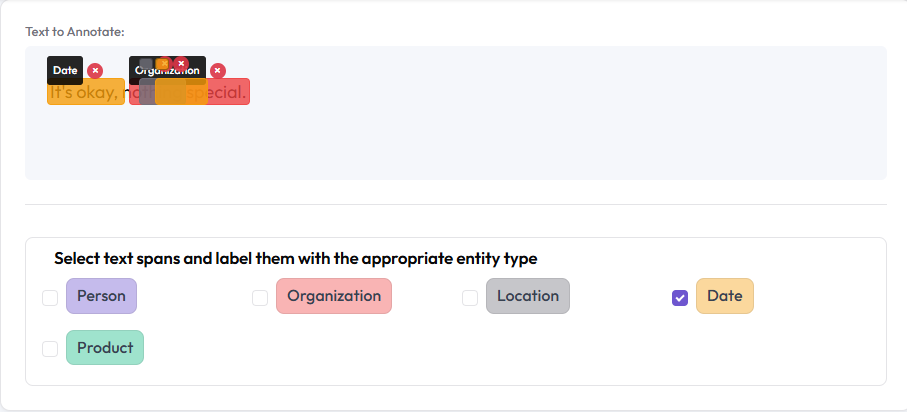
\includegraphics[width=0.95\linewidth]{./images/image_potato_span.png}
    \caption{In Potato le etichette degli span sovrapposti si accumulano nel punto di intersezione e coprono il testo.}
    \label{fig:potato}
\end{figure}

L'interfaccia qui descritta rende l'overlap un'operazione diretta. Selezionare una seconda volta una porzione di testo già annotata, con un'etichetta diversa, aggiunge un nuovo span senza rimuovere il precedente. Gli span sovrapposti vengono resi visibili con una fascia colorata per span, impilata sotto il testo in base al livello di sovrapposizione (Figura~\ref{fig:interfaccia-overlap}). L'annotatore vede a colpo d'occhio quante etichette coprono ciascuna porzione di testo, invece di doverlo ricostruire da una lista di coordinate.

\begin{figure}[H]
    \centering
    \figura[width=0.95\linewidth]{images/image 3.png}
    \caption{Gli span sovrapposti sono resi visibili da una fascia colorata impilata per ciascuno.}
    \label{fig:interfaccia-overlap}
\end{figure}

Le etichette non sono sempre visibili. Compaiono solo al passaggio del mouse, e mostrano tutti gli span che coprono il punto sotto il cursore. Il testo resta così leggibile anche con molte sovrapposizioni, al contrario di quanto avviene in Potato, dove le etichette si accumulano sopra il testo nel punto di intersezione. Nella Figura~\ref{fig:interfaccia-overlap} il cursore si trova sullo span che inizia con ``NASA'', ed è per questo che solo la sua etichetta è visibile.

Accanto all'etichetta che compare al passaggio del mouse c'è un pulsante che rimuove quello span. I confini di uno span già creato non si modificano, per correggerlo lo si rimuove e lo si ridefinisce con una nuova selezione. L'etichetta da applicare si sceglie dai pulsanti colorati sopra il testo oppure dalla tastiera, perché ogni pulsante riporta il numero che lo richiama, così che un annotatore che lavora su molti documenti non debba spostare la mano sul mouse per cambiare etichetta.

L'interfaccia non è cablata su un task predefinito, ogni componente dello schema (\S\ref{sec:schema}) corrisponde a un blocco visivo generato dinamicamente, uno per \verb|span_highlight|, uno per \verb|classification|, assemblato in base ai componenti presenti nello schema del progetto. Aggiungere un nuovo tipo di componente al sistema significa aggiungere un nuovo blocco, senza modificare quelli esistenti.

L'interazione qui descritta è ciò che rende l'overlap accessibile all'annotatore, ed è il punto in cui il lavoro di onboarding e distribuzione descritto nelle sezioni seguenti si traduce in una risposta effettiva. La sezione seguente risale ai passaggi che l'annotatore attraversa prima di arrivarci. Come quella risposta viene misurata è descritto in \S\ref{sec:live}.

% =====================================================================
\section{L'ingresso nel progetto}
\label{sec:onboarding}

La sezione precedente ha mostrato l'annotatore al lavoro. Questa descrive come ci arriva. Un annotatore che si iscrive a un progetto non riceve subito documenti da annotare. Il sistema lo fa prima attraversare una pipeline di onboarding (\S\ref{sec:annotatore}), la stessa sequenza di fasi già introdotta nel capitolo precedente, implementata come una macchina a stati.

\begin{figure}[H]
    \centering
    \figura[width=0.95\linewidth]{images/image 4.png}
    \caption{Le fasi della pipeline di onboarding, ciascuna attivabile o disattivabile in configurazione.}
    \label{fig:onboarding-fasi}
\end{figure}

Le fasi, riportate in Figura~\ref{fig:onboarding-fasi}, sono controllate da un interruttore indipendente nella configurazione del progetto, quindi un progetto minimale può disattivarle tutte e portare l'annotatore direttamente all'annotazione, mentre uno studio più esigente le attiva tutte, incluso l'obbligo di superare un task di pratica prima di procedere. Il motore che gestisce la sequenza è lo stesso in entrambi i casi. Cambia solo la configurazione.

Il contenuto di ogni fase è definito dal ricercatore, non cablato nel sistema. Lo screening è una lista di domande configurabile, caricata come file YAML o JSON, con tipi di risposta diversi (testo, numero, scelta singola o multipla) e domande obbligatorie o facoltative, utili non solo per eleggibilità e demografia di base ma anche per domande personalizzate specifiche dello studio. Codebook e istruzioni sono invece documenti liberi in Markdown, caricati allo stesso modo. La validazione dei file caricati è descritta in \S\ref{sec:configurazione}.

L'annotatore entra da un link che contiene il suo identificativo sulla piattaforma di reclutamento e quello del progetto. Se il progetto non è attivo, il sistema rifiuta la sessione. Altrimenti restituisce la fase da cui l'annotatore deve partire. L'avanzamento nella pipeline è registrato nell'iscrizione dell'annotatore (\S\ref{sec:annotatore}), non nel client. Un annotatore che torna a metà pipeline riprende da dove aveva lasciato.

La prima fase è il consenso informato. L'annotatore legge il testo preparato dal ricercatore e lo accetta prima di procedere (Figura~\ref{fig:consenso}).

\begin{figure}[H]
    \centering
    \figura[width=0.70\linewidth]{images/consenso.png}
    \caption{Il consenso informato, con il testo definito dal ricercatore, va accettato prima di proseguire.}
    \label{fig:consenso}
\end{figure}

Segue lo screening, con le domande definite dal ricercatore (Figura~\ref{fig:screening}). Se manca una risposta obbligatoria, il server rifiuta l'invio.

\begin{figure}[H]
    \centering
    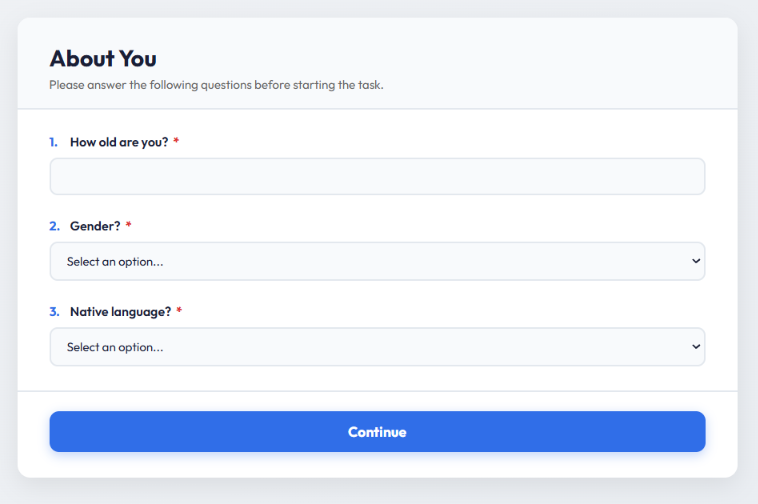
\includegraphics[width=0.70\linewidth]{images/Screening.png}
    \caption{Il questionario di screening, con domande definite dal ricercatore per lo studio specifico.}
    \label{fig:screening}
\end{figure}

Il codebook presenta il quadro teorico dello studio, per esempio le definizioni delle categorie da annotare. L'annotatore lo legge e conferma di averlo fatto prima di passare alle istruzioni (Figura~\ref{fig:codebook}).

\begin{figure}[H]
    \centering
    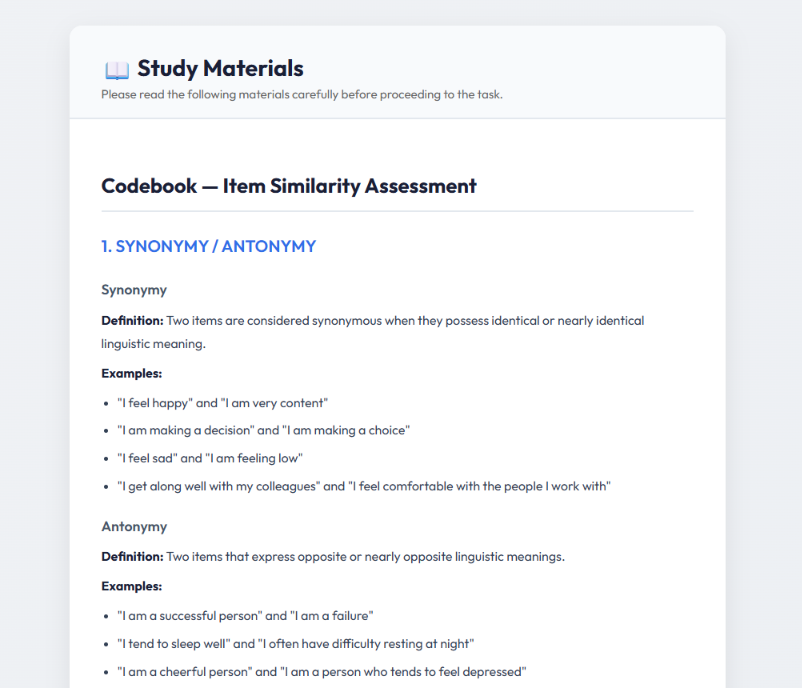
\includegraphics[width=0.70\linewidth]{images/Codebook 1.png}
    \caption{Il codebook presenta il quadro teorico dello studio, e l'annotatore conferma di averlo letto.}
    \label{fig:codebook}
\end{figure}

Le istruzioni spiegano come svolgere il task. Se il ricercatore lo prevede, sono seguite da un task di pratica. L'annotatore annota un testo di esempio con la stessa interfaccia della sezione precedente e riceve subito un riscontro (Figura~\ref{fig:pratica}). Per ogni span della soluzione vede se l'ha individuato, per la classificazione vede la risposta corretta, e può leggere i suggerimenti preparati dal ricercatore. Il confronto con la soluzione avviene nel browser e usa lo stesso criterio delle gold unit, descritto in \S\ref{sec:live}. Se il task di pratica è obbligatorio, l'annotatore deve riprovare finché non risponde correttamente. Altrimenti può proseguire anche dopo un tentativo sbagliato.

\begin{figure}[H]
    \centering
    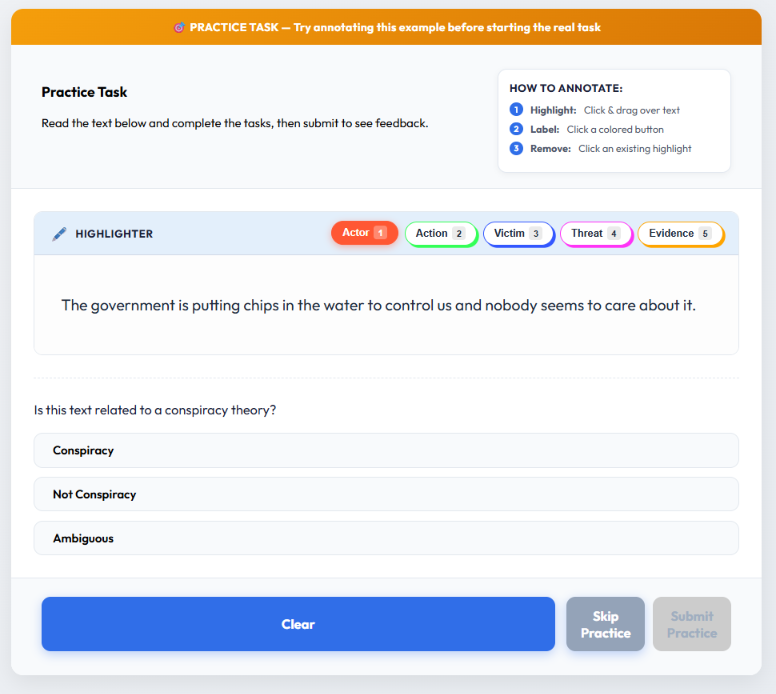
\includegraphics[width=0.70\linewidth]{images/Practice Task .png}
    \caption{Il riscontro sul task di pratica indica quali span della soluzione sono stati individuati.}
    \label{fig:pratica}
\end{figure}

Superato l'onboarding, l'annotatore riceve i documenti da annotare. Come il sistema li distribuisce è una scelta del ricercatore, descritta in \S\ref{sec:configurazione}. Con l'ingresso nel progetto si chiude il percorso dell'annotatore. Le prossime due sezioni cambiano prospettiva, dal lavoro dell'annotatore a quello del ricercatore che lo rende possibile. La prima descrive come il ricercatore sorveglia uno studio in corso, la seconda come lo configura senza scrivere codice.

% =====================================================================
\section{Amministrazione del task live}
\label{sec:live}
\label{sec:qualita}

Il sistema è pensato perché il ricercatore possa configurare e sorvegliare uno studio senza competenze tecniche, un obiettivo che vale sia in fase di configurazione iniziale sia oltre, quando lo studio è già in corso. Questa sezione parte dal secondo caso. Mentre gli annotatori lavorano, il ricercatore ha bisogno di sapere a che punto è la raccolta, se i dati sono di qualità sufficiente e come intervenire se qualcosa non va. Il punto di partenza è la dashboard del progetto (Figura~\ref{fig:dashboard}).

% TODO: aggiungere sullo screenshot i numeri (1) stato, (2) transizioni, (3) avanzamento, (4) conteggi
\begin{figure}[H]
    \centering
    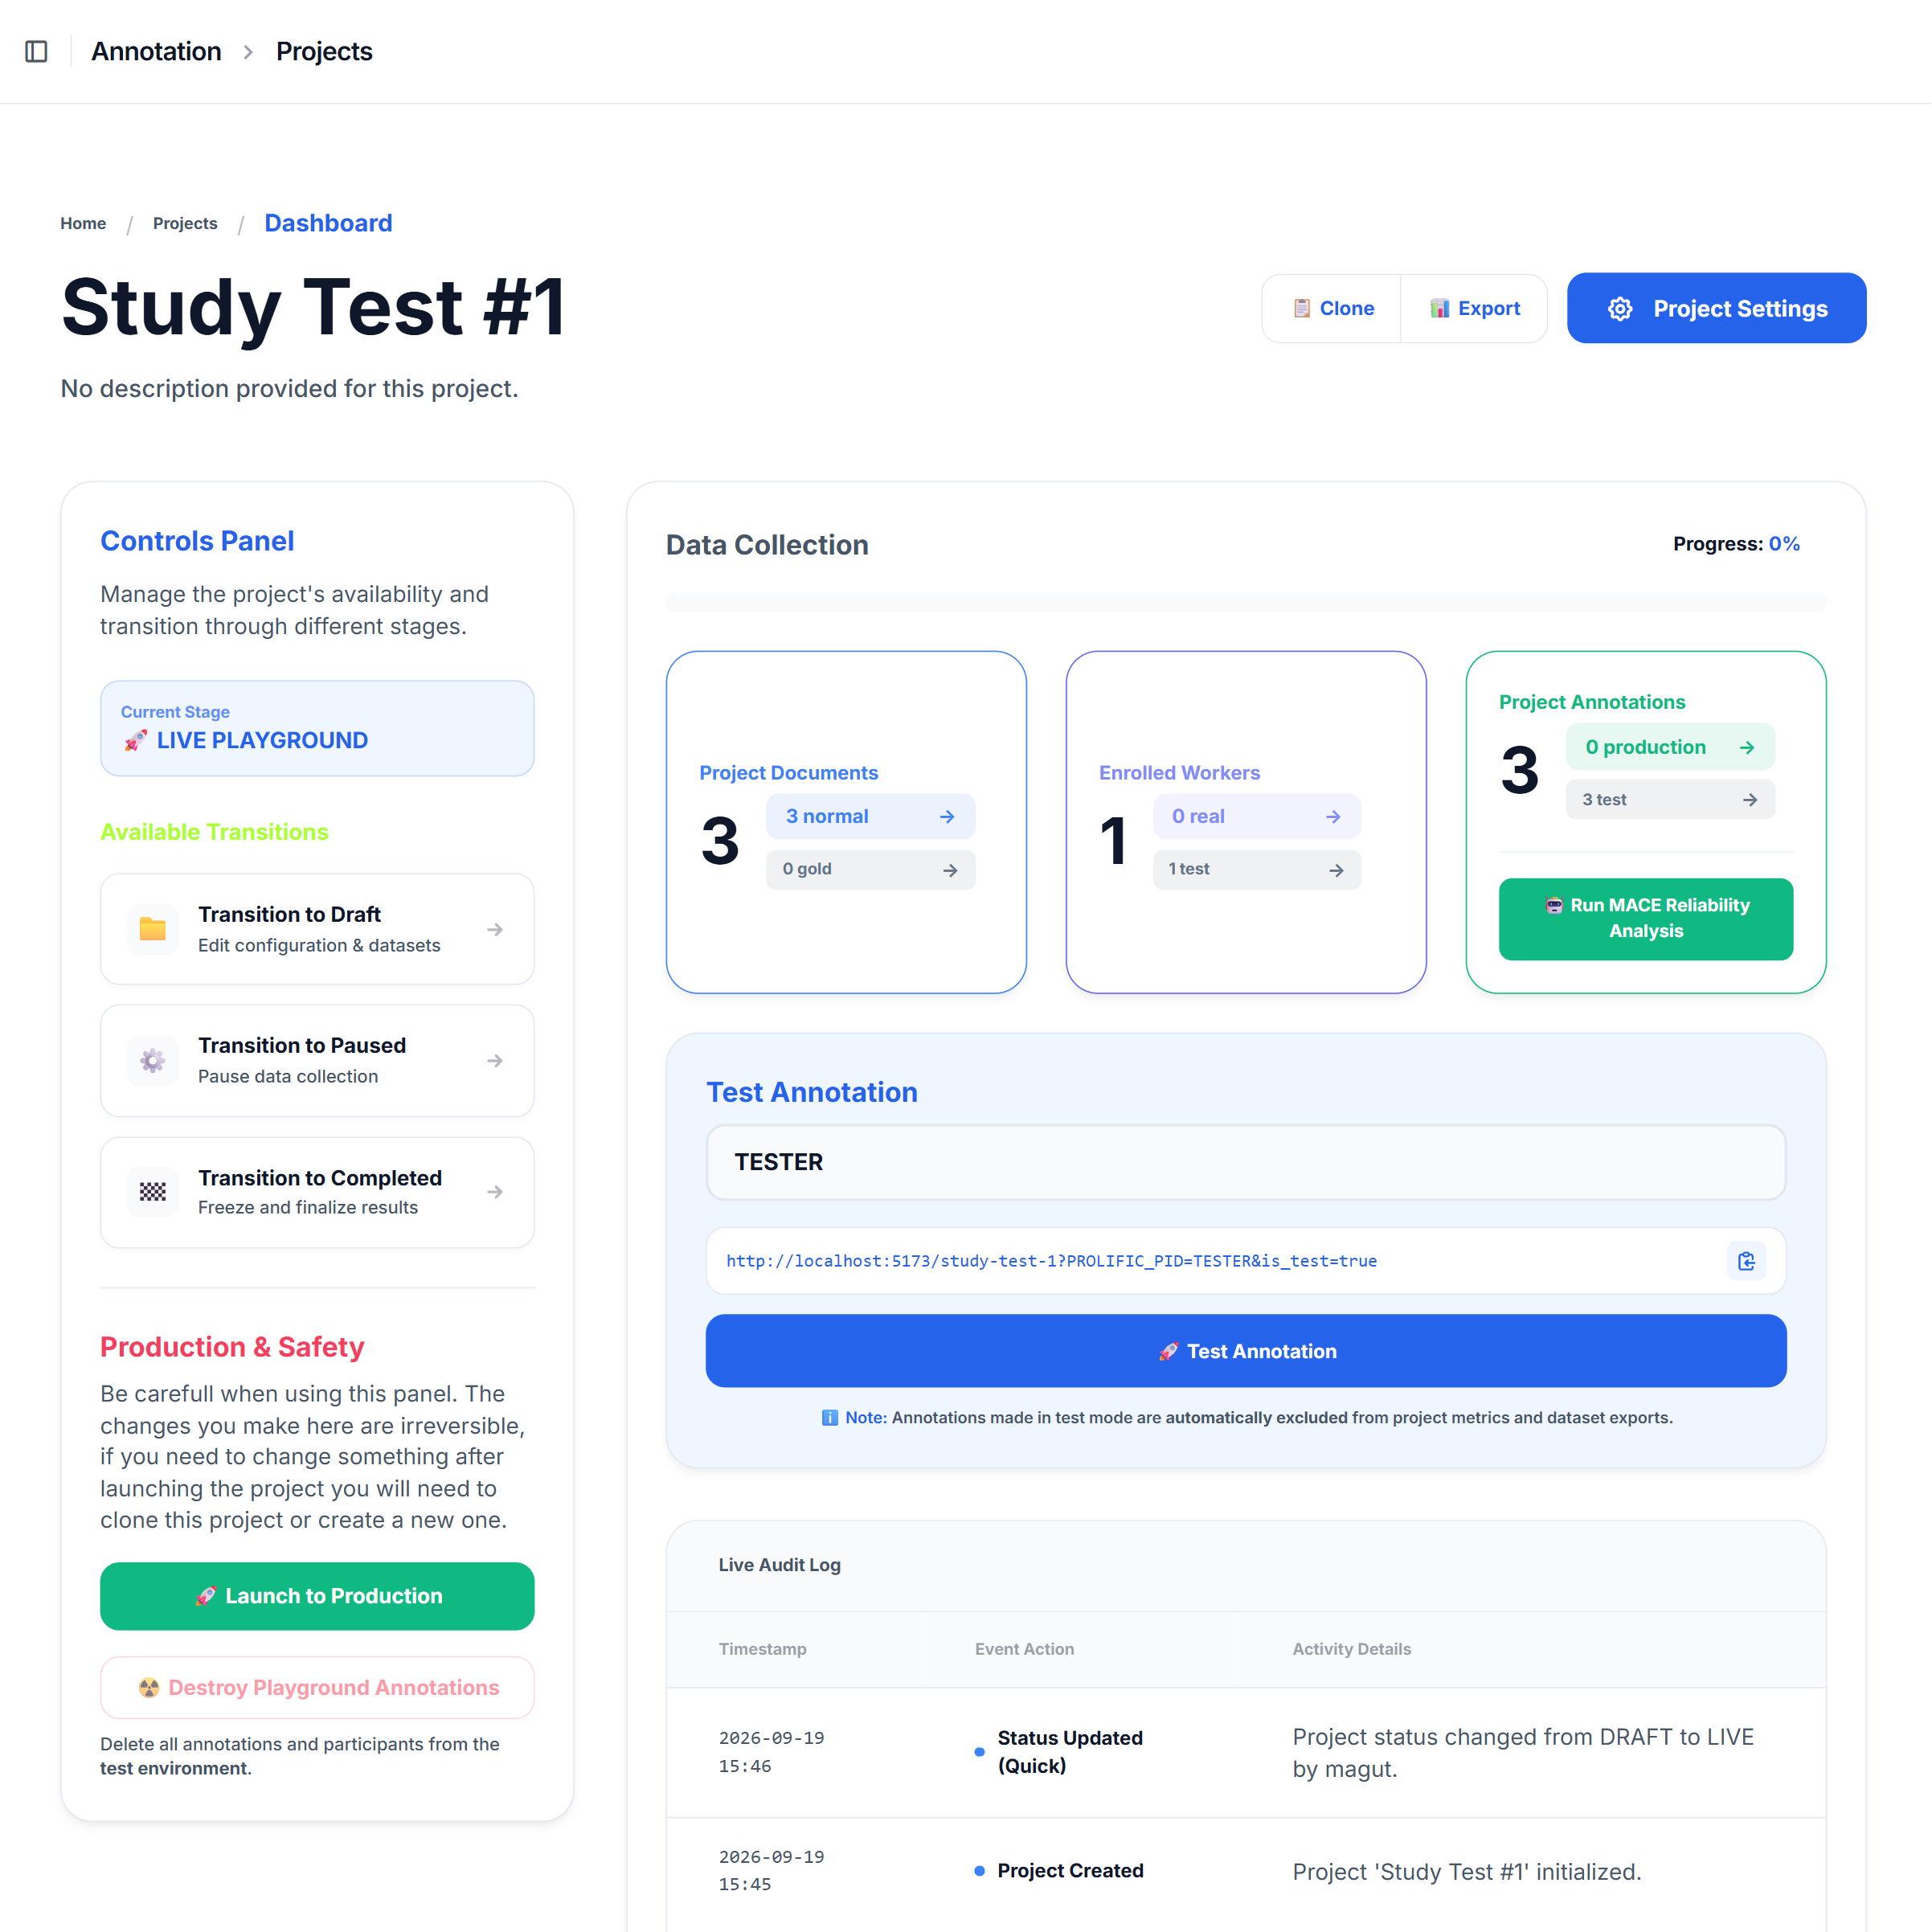
\includegraphics[width=1\linewidth]{images/Dashboard white cut.png}
    \caption{La dashboard del progetto. I riquadri numerati indicano lo stato corrente (1), le transizioni disponibili (2), l'avanzamento della raccolta (3) e i conteggi di documenti, gold unit, annotatori e annotazioni (4).}
    \label{fig:dashboard}
\end{figure}

Il primo strumento è lo stato del progetto, definito nel capitolo precedente (\S\ref{sec:progetto}). La dashboard mostra lo stato corrente (1) e le transizioni disponibili (2). Lo stato decide cosa vedono gli annotatori. Solo un progetto attivo accetta sessioni e assegna documenti. Negli altri stati il sistema rifiuta le nuove sessioni, e chi sta annotando riceve un messaggio che avvisa che il progetto non accetta più annotazioni. Quando il progetto è attivo, il ricercatore può aprirlo dall'amministrazione come partecipante di prova e percorrere tutta la pipeline. Finché il progetto resta in modalità playground, cioè attivo ma non ancora pubblicato ufficialmente, tutte le sessioni vengono registrate come prova. Le annotazioni di prova sono conteggiate separatamente da quelle reali e non entrano nella valutazione sulle gold unit. Al momento della pubblicazione ufficiale il sistema cancella tutte le annotazioni e le iscrizioni raccolte fino a quel momento, e la raccolta reale parte da zero.

La dashboard riporta anche l'avanzamento della raccolta (3), calcolato sul numero di annotazioni ricevute rispetto a quelle richieste dai documenti, insieme al numero di documenti, gold unit, annotatori iscritti e annotazioni raccolte (4).

Le risposte raccolte attraverso l'interfaccia descritta in \S\ref{sec:overlap} sono ciò che il sistema misura per stimare la qualità del lavoro di un annotatore. Tra i documenti distribuiti (\S\ref{sec:distribuzione}) figurano anche le gold unit (\S\ref{sec:goldunit}). Il sistema le usa per misurare la qualità delle risposte raccolte, con due meccanismi complementari.

Il primo è l'iniezione periodica di gold unit nel flusso di documenti regolari, con una frequenza configurabile per ogni progetto. Quando un annotatore riceve una gold unit, la sua risposta viene confrontata con la soluzione nota componente per componente. La classificazione richiede corrispondenza esatta, mentre gli span richiedono che la soluzione trovi un corrispondente nella risposta dell'annotatore entro una tolleranza di cinque caratteri sui confini.

L'esito di ogni gold unit aggiorna l'accuratezza cumulata dell'annotatore su quel progetto specifico. La decisione di escludere un annotatore è delegata a una strategia di valutazione, isolata dal resto del sistema, che esclude l'annotatore quando l'accuratezza scende sotto una certa soglia configurabile, dopo un numero minimo di gold unit completate. Un annotatore escluso non riceve più documenti e viene avvisato dell'esclusione. La separazione tra meccanismo di iniezione e criterio di esclusione lascia aperta la possibilità di modificare il criterio senza toccare il resto della pipeline di controllo qualità. Il ricercatore vede per ogni iscrizione l'accuratezza raggiunta e lo stato dell'annotatore (Figura~\ref{fig:iscrizioni}).

\begin{figure}[H]
    \centering
    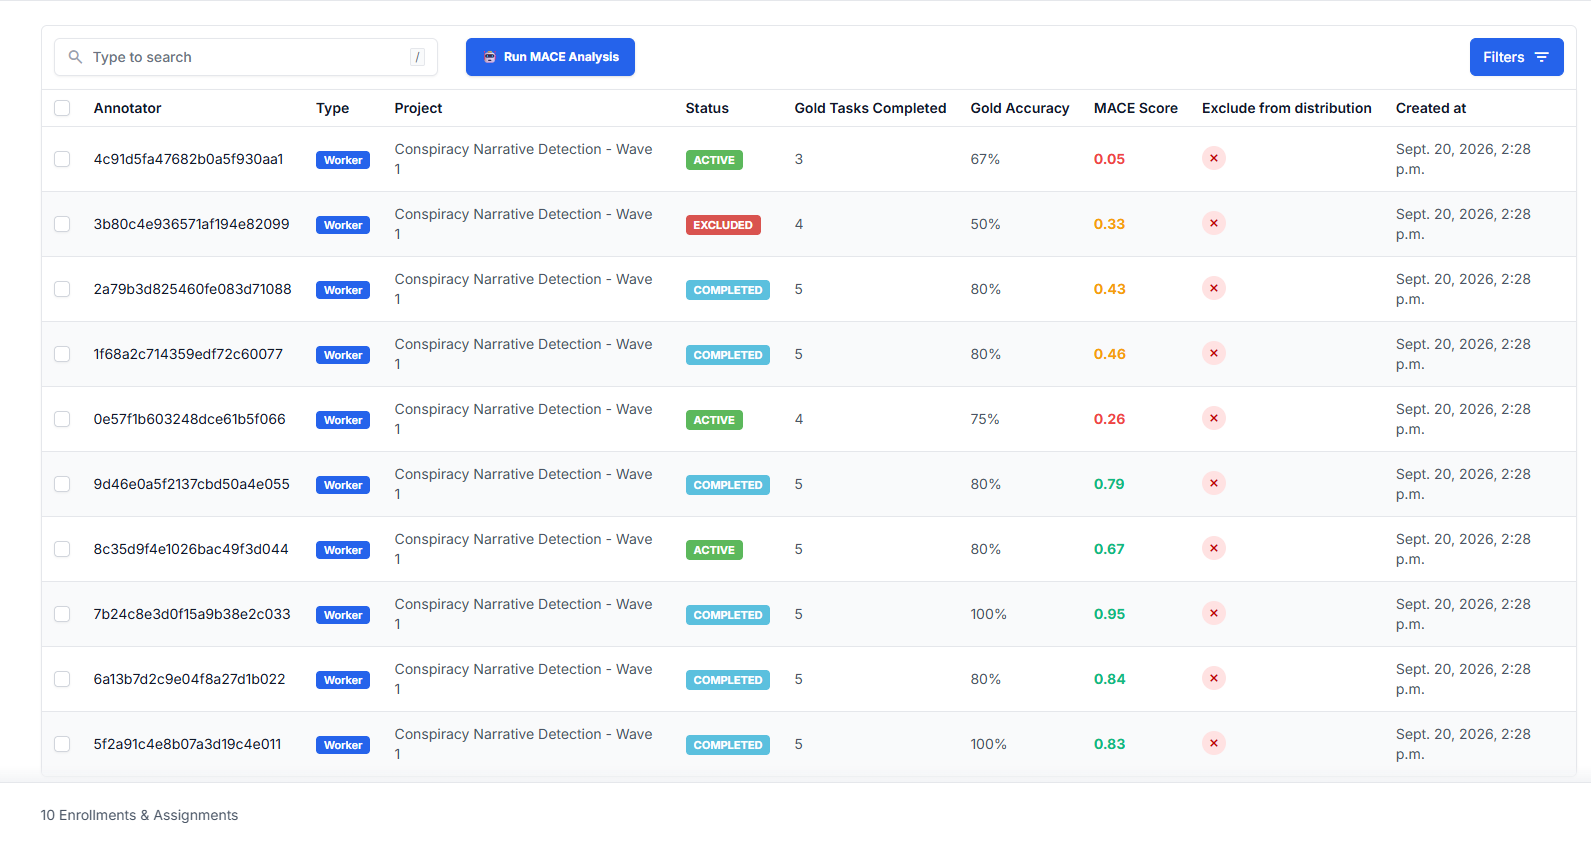
\includegraphics[width=1\linewidth]{images/Annotation Mace Gold.png}
    \caption{Per ogni iscrizione il ricercatore vede accuratezza sulle gold unit, stato e punteggio MACE.}
    \label{fig:iscrizioni}
\end{figure}

Il secondo meccanismo è l'integrazione di MACE (Multi-Annotator Competence Estimation) \parencite{hovy2013mace}, un algoritmo Expectation-Maximization che stima congiuntamente l'etichetta più probabile per ciascun documento e la competenza di ciascun annotatore, a partire dalle sole annotazioni raccolte, senza il coinvolgimento delle gold unit.

Il ricercatore lancia il calcolo MACE dalla console di amministrazione su un progetto. Il sistema produce due output distinti. Il primo è l'etichetta stimata e la confidenza associata per ogni documento, il secondo è un punteggio di competenza sull'iscrizione al progetto per ogni annotatore (\S\ref{sec:annotatore}). Il primo output è una stima di affidabilità complementare alle gold unit, utile dove la loro copertura è limitata; il secondo estende la valutazione dell'annotatore oltre le sole gold unit esplicite, usando l'intero volume di annotazioni raccolte.

Gold unit e MACE misurano la qualità dopo la raccolta. Quando invece qualcosa va cambiato c'è un vincolo. Una volta pubblicato ufficialmente un progetto, la sua configurazione e il suo dataset non sono più modificabili, così che tutti gli annotatori lavorino nelle stesse condizioni.

Per permettere al ricercatore di modificare un campo mentre il progetto è già pubblicato, può duplicare il progetto in tre modalità, solo configurazione, configurazione e dataset completo, oppure configurazione con le gold unit, i documenti che non hanno ancora raggiunto il numero minimo di annotazioni e gli annotatori non esclusi e non ancora completati, di cui vengono azzerate le metriche sulle gold unit, per iterare rapidamente su varianti dello studio senza ricostruire la configurazione da zero. La copia parte sempre in bozza e non pubblicata.

Stati, soglie di esclusione e parametri di distribuzione che il ricercatore osserva durante la raccolta vengono però decisi prima del lancio. La sezione seguente descrive come.

% =====================================================================
\section{Configurazione del task}
\label{sec:configurazione}
\label{sec:distribuzione}
\label{sec:amministrazione}

Prima che un progetto raccolga dati, il ricercatore ne definisce ogni aspetto. L'intera configurazione descritta in questo capitolo, schema, dataset, pipeline di onboarding, strategia di distribuzione, controllo qualità, è esposta attraverso un'amministrazione Django estesa, organizzata in schede tematiche: Project Details, Dataset Upload, Annotation Schema, Screening Setup, Codebook Setup, Instruction, Practice Task, Quality \& Monitoring, Distribution (Figura~\ref{fig:schede}).

\begin{figure}[H]
    \centering
    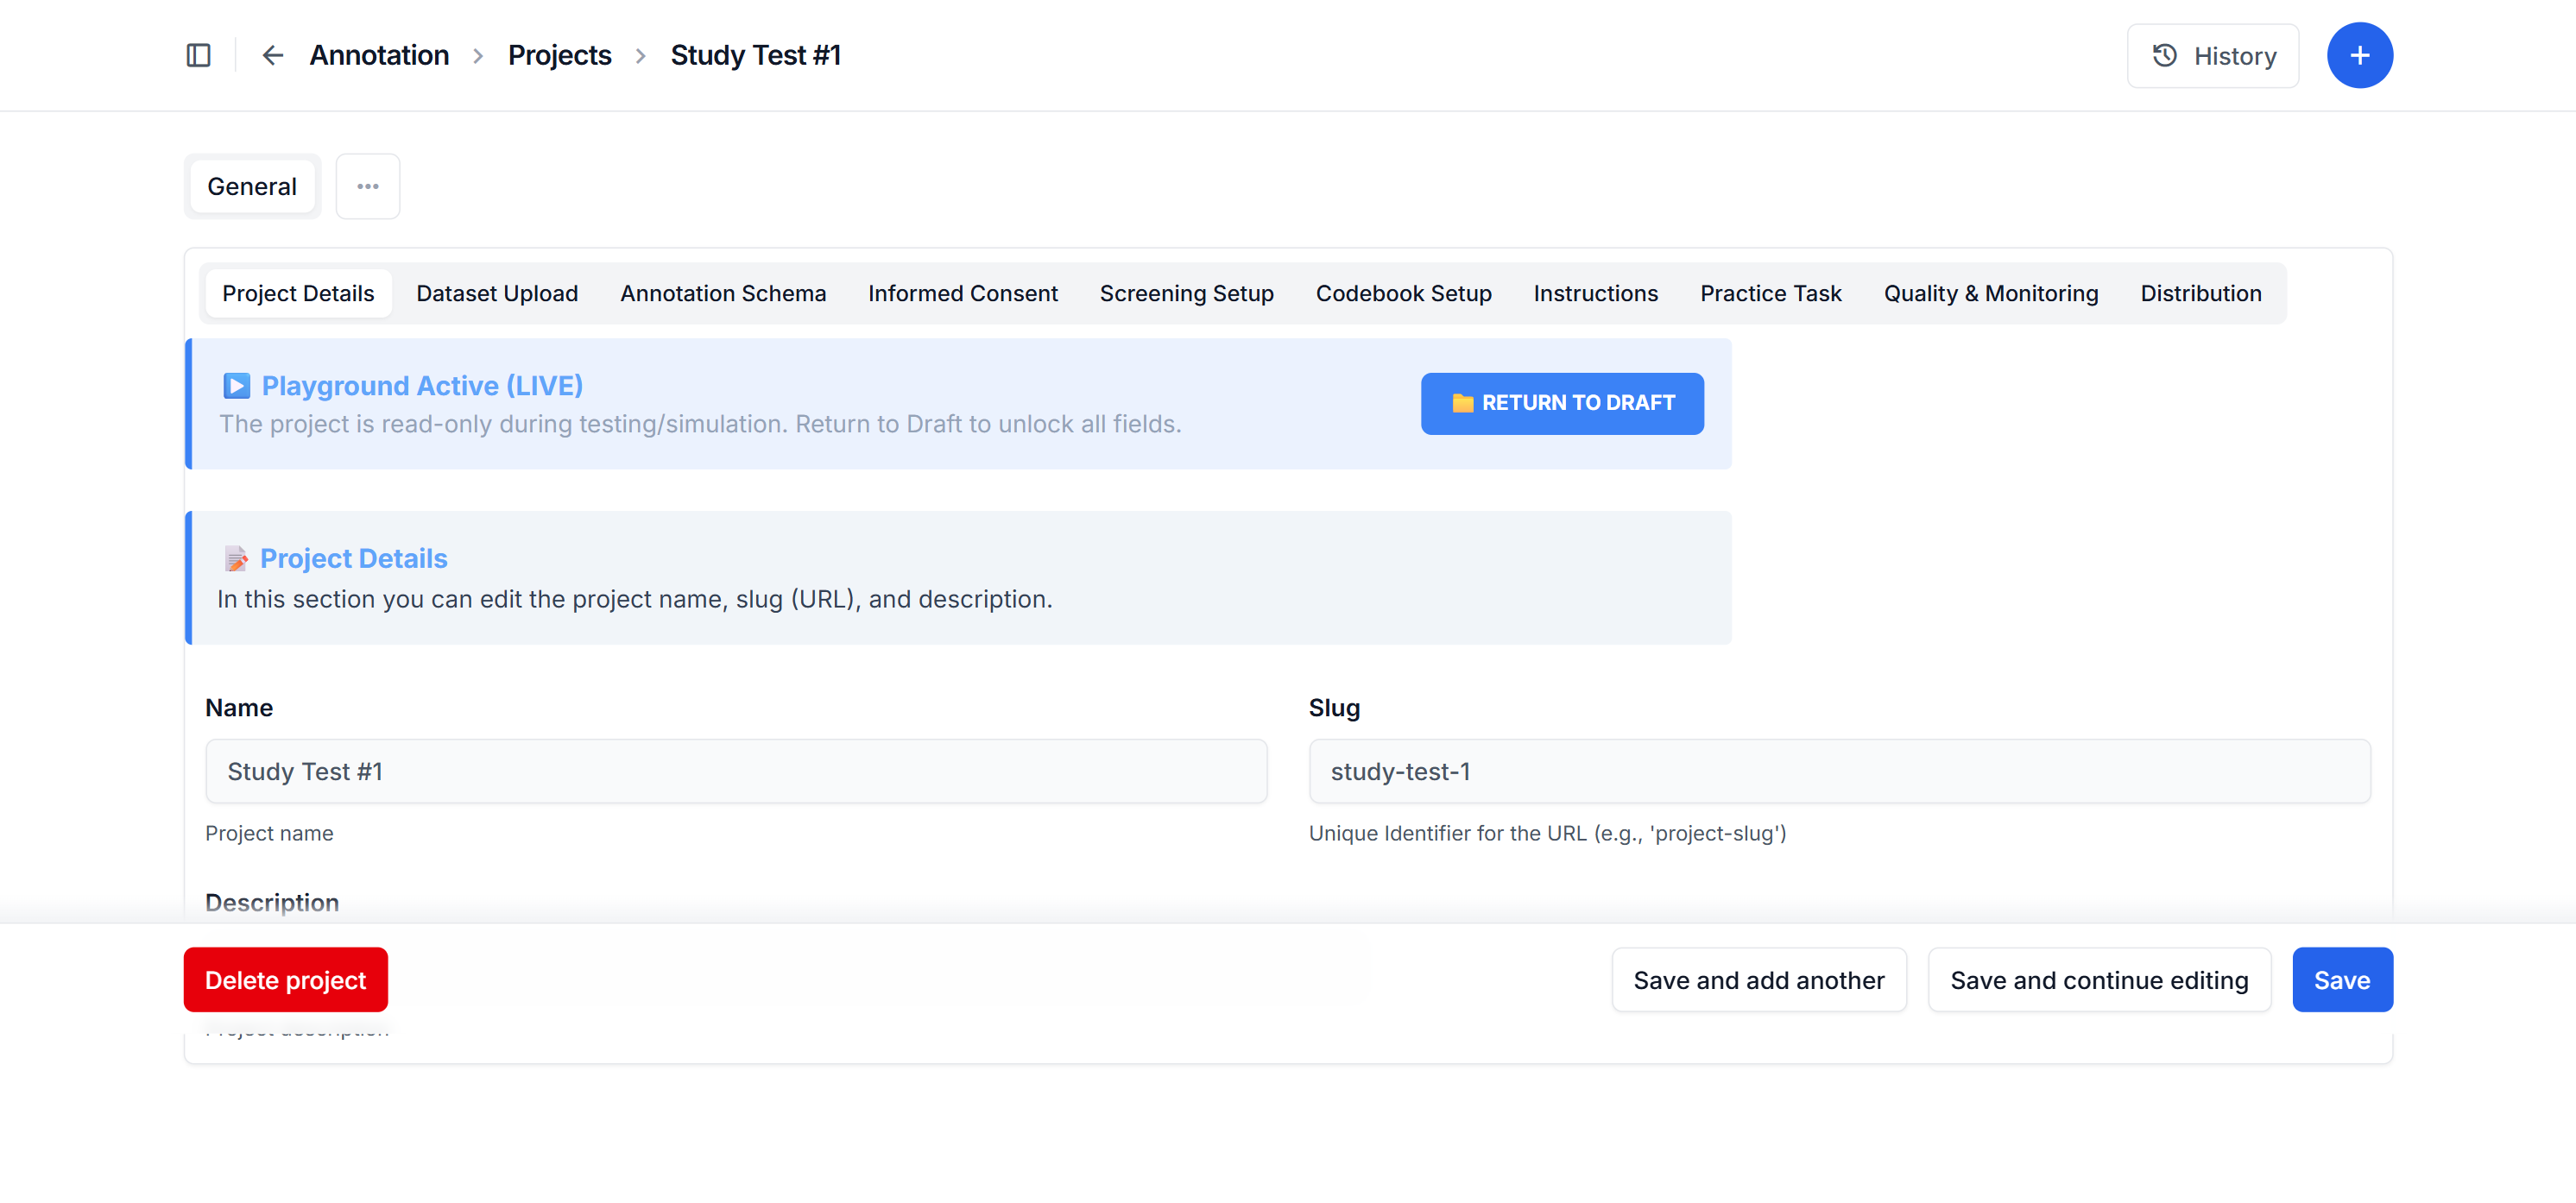
\includegraphics[width=1\linewidth]{images/panel dashboard.png}
    \caption{La configurazione del progetto è divisa in schede tematiche, una per ogni aspetto dello studio.}
    \label{fig:schede}
\end{figure}

Schema, screening, codebook e istruzioni si caricano come file YAML o Markdown. Lo schema viene validato nella sua struttura e rifiutato se non conforme, il task di pratica viene bloccato se la sua soluzione non è compatibile con lo schema, mentre lo screening viene solo letto come YAML o JSON e i testi in Markdown vengono salvati così come sono. Un errore nello schema o nel task di pratica viene quindi segnalato prima che il progetto possa essere pubblicato, non scoperto a raccolta dati in corso.

Una volta che un annotatore ha superato l'onboarding (\S\ref{sec:onboarding}), il sistema deve decidere quali documenti assegnargli. Lo fa secondo una di tre strategie, selezionabile per progetto. La strategia standard assegna documenti in modo casuale, entro una soglia minima e massima di annotazioni per documento. La strategia a piena sovrapposizione espone a ogni annotatore l'intero dataset, per studi che richiedono la massima ridondanza. La strategia a blocchi con annotatori fissi divide il dataset in blocchi di dimensione configurabile e assegna ciascun blocco a un numero fisso di annotatori, con una ridondanza controllata. È utile quando si vuole misurare il livello di accordo tra un gruppo chiuso di annotatori sugli stessi documenti.

L'assegnazione può coinvolgere più annotatori che richiedono un documento nello stesso istante. Per questo avviene sotto lock a livello di record nel database, il documento somministrato resta bloccato per tutta la durata della transazione, così che due richieste concorrenti non ricevano mai lo stesso documento.

Una volta distribuiti, i documenti includono anche le gold unit (\S\ref{sec:goldunit}). Il ricercatore le carica nella stessa amministrazione e fissa i parametri del controllo qualità descritto in \S\ref{sec:live}, cioè ogni quanti documenti iniettarne una, l'accuratezza minima richiesta e il numero di gold unit dopo cui la valutazione comincia.

Configurazione e amministrazione sono la superficie che il ricercatore vede. L'ultima sezione del capitolo scende sotto quella superficie, nell'architettura che la rende possibile.

% =====================================================================
\section{Architettura del sistema}
\label{sec:architettura}

Interfaccia di annotazione (\S\ref{sec:overlap}) e amministrazione (\S\ref{sec:live}, \S\ref{sec:configurazione}) sono le due facce del sistema che rispettivamente l'annotatore e il ricercatore vedono. Quello che le rende entrambe possibili è descritto qui. Il sistema è composto da un backend Django, che espone un'API REST e la console di amministrazione, e da un frontend Vue 3 single page, che implementa l'interfaccia di annotazione. I due componenti vengono eseguiti in container Docker separati, con PostgreSQL come base dati. Il deploy dell'intero sistema avviene con un unico comando Docker Compose, per non richiedere al ricercatore competenze di configurazione infrastrutturale.

\begin{figure}[H]
    \centering
    \figura[width=0.75\linewidth]{images/diagram.jpg}
    \caption{Il backend espone due piani separati, configurazione per il ricercatore ed esecuzione per l'annotatore, entrambi alimentati dallo stesso schema di annotazione.}
    \label{fig:architettura}
\end{figure}

L'architettura, schematizzata in Figura~\ref{fig:architettura}, separa nettamente due piani, il primo quello di configurazione, esposto tramite la dashboard di amministrazione Django, rivolto al ricercatore e ai suoi collaboratori, e il secondo di esecuzione, esposto tramite API REST e rivolto all'annotatore. Configurare l'annotazione e comporla non richiedono le stesse competenze, né la stessa superficie di rischio, e vanno perciò esposte separatamente. I due piani condividono un solo punto di verità, lo schema di annotazione del progetto (\S\ref{sec:schema}), che alimenta sia la validazione lato configurazione sia la generazione dell'interfaccia lato esecuzione. Un cambiamento allo schema si riflette in entrambi senza sincronizzazione manuale.

Backend, frontend e i due piani che espone sono l'infrastruttura su cui si appoggia tutto quello che il capitolo ha descritto finora. Con questo il capitolo chiude la descrizione dei meccanismi che realizzano i concetti del capitolo precedente (\S\ref{cap:dati}). Il capitolo Risultati ne valuta il funzionamento messo alla prova.

\chapter{Risultati}
\label{chap:risultati}

\chapter{Discussione}
\label{chap:discussione}

\chapter{Limitazioni e Sviluppi Futuri}
\label{chap:limitazioni}

\chapter{Conclusioni}
\label{chap:conclusioni}

\printbibliography

\backmatter
\cleardoublepage
\phantomsection
\addcontentsline{toc}{chapter}{\bibname}

\end{document}